\documentclass[12pt]{article}
\usepackage[margin=1in]{geometry}
\usepackage{amsmath, amssymb, amsthm, graphicx, hyperref}
\usepackage{subfigure}
\usepackage{color}
\usepackage{fancyhdr}
\usepackage{multirow, multicol}
\usepackage{pdfpages}
\usepackage{stfloats}
\usepackage{tikz}
\pagestyle{fancy}
\pagestyle{empty}
\usepackage{amsmath,amssymb,latexsym,epsfig,tikz}
\usepackage{graphicx}
\usepackage{subfigure}
\usepackage{pgfplots}
\usepackage{tikz}
\textwidth 7in
\oddsidemargin -0.25in
\topmargin-0.80in
\textheight 9.5in


\fancypagestyle{firststyle}
{
  \renewcommand{\headrulewidth}{0pt}
  \fancyhead[LO]{\includegraphics{nyu_short_black}}
  \fancyhead[RO]{}
	\fancyfoot{}
}

%\fancyhead[LO]{\scalebox{0.25}{\includegraphics{nyu_short_black}}}
\fancyhead[RO]{\tiny Math-UA.121.A}


%\fancyfoot[RO]{\begin{tikzpicture}
%[scale=1, line/.style={black}]
%\draw[line] (0, 0)--(2,0)--(2, 2)--(0, 2)--(0, 0);
%%\node at (-0.5, 1) [anchor=east]{\large Score};
%\end{tikzpicture}}

\newcommand*\mycirc[1]{%
  \begin{tikzpicture}[baseline=(C.base)]
    \node[draw,circle,inner sep=1pt](C) {#1};
  \end{tikzpicture}}

\newcommand{\R}{\mathbb{R}}
\newcommand{\E}{\mathbb{E}}
\newcommand{\proj}{\textbf{proj}}
\newcommand{\curl}{\textrm{curl }}
\newcommand{\divergence}{\textrm{div }}
% For boldface vectors:
\renewcommand{\vec}[1]{\mathbf{#1}}
\renewcommand\arraystretch{1.6}

\begin{document}

\begin{enumerate}
\item Suppose $f$ is a differentiable function with values as shown. What is $\displaystyle (f^{-1})'(0)$?  

\begin{multicols}{2}
	\begin{tabular}{r|c|c|c|c}
	$x$ & 0 & 1 & 2 & 3 \\
	\hline
	$f(x)$ & 4 & 2 & 0 & -2 \\
	\hline
	$f'(x)$ & $0$ & $-1$ & $-2$ & $-4$ 
	\end{tabular}
	\columnbreak
	\begin{enumerate}\setlength{\itemsep}{.4 cm}
	\item[(A)] $-\frac13$
	\item[(B)] $-\frac12$
	\item[(C)] $-3$
	\item[(D)] $-2$
	\item[(E)] $\frac12$
	\end{enumerate}
\end{multicols}

\vspace{0.1cm}


\item Suppose that $f(x) = \displaystyle \int_{x}^{2} \cos(t^2) \ dt$.  What is $f'(x)$?

\begin{enumerate}
\item[(A)] $\cos(x^2)$
\item[(B)] $\displaystyle \frac{\sin (x^2)}{2x}$
\item[(C)] $-2x\sin(x^2)$
\item[(D)] $-\cos (x^2)$
\item[(E)] None of the above
\end{enumerate}


\item A car is traveling on a straight road, with a velocity given by the graph below.  Here, velocity is measured in miles per hour and time is measured in hours.  Positive velocity means movement to the right, negative velocity means movement to the left.

What is the displacement of the car in miles during the time period $0 \leq t \leq 5$ ?



\begin{center}
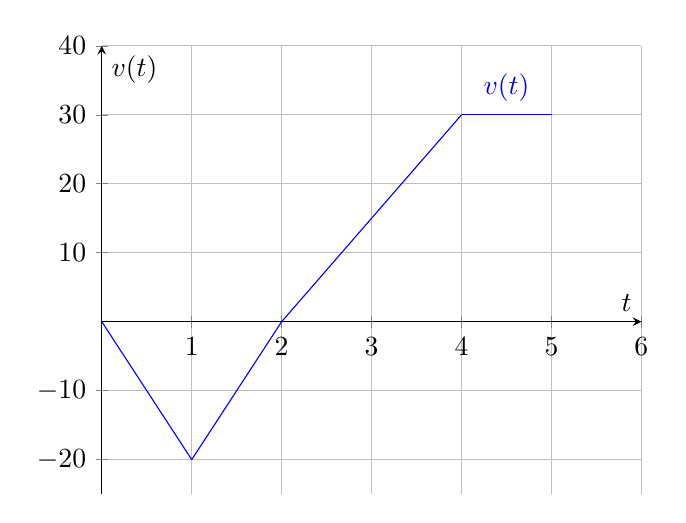
\begin{tikzpicture}
\begin{axis}[grid=both,
	axis x line=middle,
	axis y line=center,
	xmin=0,
	xmax=6,
	ymin=-25,
	ymax=40,
	xlabel=$t$,ylabel=$v(t)$,
	xtick={0,1,2,3,4,5,6},
	ytick={-20,-10,10,20,30,40}
]
\addplot[blue,mark=none,
	 domain=0:1,samples=100]
	{-1*20*x};
\addplot[blue,mark=none,
	 domain=1:2,samples=100]
	{20*(x-2)};
\addplot[blue,mark=none,
	 domain=2:4,samples=100]
	{15*(x-2)};

	\addplot[blue,mark=none,
	 domain=4:5,samples=100]
	{30};


	\node[blue] at (axis cs:4.5,34){$v(t)$};
\end{axis}	
\end{tikzpicture}
\end{center}
\begin{enumerate}
\item[(A)] There is not enough information to find the displacement
\item[(B)] $40$ miles
\item[(C)] $60$ miles
\item[(D)] $80$ miles
\item[(E)] None of the above
\end{enumerate}


\item Let $f'$ be the function graphed below.  On which of the following interval is $f$ decreasing?
\begin{center}
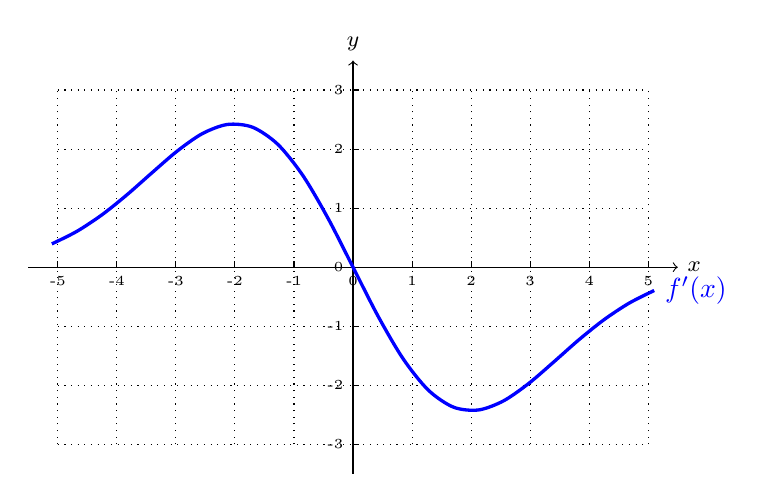
\begin{tikzpicture}[scale=0.75]
\foreach \x in {-5, -4, ..., 5}
{
	\draw[thin, dotted] (\x, -3) -- (\x, 3);
}
\foreach \y in {-3, -2, ..., 3}
{
	\draw[thin, dotted] (-5, \y) -- (5, \y);
}

\foreach \x in {-5, -4, ..., 5}
{
	\draw (\x, 0.1) -- (\x, 0) node[anchor=north]{\tiny \x};
}

\foreach \y in {-3, -2, ..., 3}
{
	\draw (0.1, \y) -- (0, \y) node[anchor=east]{\tiny \y};
}

\draw[->] (-5.5, 0) -- (5.5, 0) node[anchor=west]{\footnotesize$x$};
\draw[->] (0, -3.5) -- (0, 3.5) node[anchor=south]{\footnotesize$y$};

\draw[variable=\x, domain= -5.1:5.1, smooth, very thick, blue] plot ({\x}, {-2*\x*exp(-\x*\x/8)}) node[anchor=west]{$f'(x)$};
\end{tikzpicture}
\end{center}
\begin{multicols}{2}
\begin{enumerate}
\item[(A)] $(-5,-2)$
\item[(B)] $(0, 2 )$
\item[(C)] $(0, 5)$
\item[(D)] $(-2, 2)$
\item[(E)] None of the above
\end{enumerate}
\end{multicols}


\item Suppose that $\displaystyle \int_{-2}^{3} f(x) \ dx = 2$ and $\displaystyle \int_{3}^{5} f(x) \ dx =- 3$.  

Which one of the following statements about $f(x)$ must be true?
\begin{multicols}{2}
\begin{enumerate}
\item[(A)] $\displaystyle \int_{2}^{-3} f(x) \ dx = -2 $
\item[(B)] $\displaystyle \int_{5}^{-2} f(x) \ dx = 1$
\item[(C)] $f(x) \leq 0$ for $3 \leq x \leq 5$
\item[(D)] $\displaystyle \int_{-2}^{5} f(x) \ dx = 5$
\item[(E)] None of the above
\end{enumerate}
\end{multicols}

\vspace{1cm}



\end{enumerate}

\end{document}
